\chapter{Eschatologie musulmane}

La question eschatologique est fondamentale. Rappelez-vous, Muḥammad a
commencé la transmission des sourates avec cet appel à la conversion car
la fin des temps est proche. Nous y consacrerons un chapitre. Mais que
se passe-t-il après la mort~? Quelle est donc la théologie des fins
dernières de l'islam~?

Notons d'ores et déjà que les Traités d'eschatologie musulmane à
l'exemple du \emph{Livre de la mort et de l'au-delà}, d'al-Ġazālī
distinguent plusieurs étapes~: celle du Jour de la Résurrection, celle
du Jour Grand Rassemblement, celle du Jour du Jugement. On y décrit
l'enfer, le paradis, mais aussi un lieu étrange~: \emph{al-a`rāf}, sorte
de lieu transitoire.


\subsection{Bibliographie}

Emilio \textsc{Platti}, \emph{Islam\ldots{} étrange~?}, Paris Cerf, p.
65-71.

Sur la résurrection en islam~: l'article de Maurice \textsc{Borrmans},
«~Resurrection~», dans Jane Dammen \textsc{McAuliffe} (ed.)
\emph{Encyclopedia of the Qur'ân}, Leiden, Boston, Brill, 2004,
p.434-435 est une très bonne synthèse pour la dimension coranique. À
noter la récente réédition du classique, paru initialement en 1981, de
Jane Idleman \textsc{Smith}, Yvonne \textsc{Yazbeck Haddad,}


\emph{The
Islamic Understanding of Death and Resurrection}, Oxford, Oxford
University Press, 2002² qui donne une vision plus large intégrant les
données de la \emph{Sunna}, des écoles du \emph{kalâm} et de la
mystique. 

Enfin, Louis \textsc{Gardet}, \emph{Dieu et la destinée de
l'homme,} p. 231-346 propose un développement des questions
eschatologiques relevées par le \emph{kalām} mais la présentation reste
assez éloignée des manuels traditionnels de l'islam pour épouser
principalement les problématiques de la théologie chrétienne. \\


L'eschatologie musulmane est traversée par plusieurs étapes à l'issue
desquelles l'homme est destiné à se rendre dans une des demeures.

\vide{i.-les-uxe9tapes-dans-lau-deluxe0}{%
\section{Les étapes dans
l'au-delà}\label{i.-les-uxe9tapes-dans-lau-deluxe0}}

\vide{le-jour-de-la-ruxe9surrection}{%
\subsection{Le Jour de la
Résurrection}\label{le-jour-de-la-ruxe9surrection}}

On trouve soixante-dix occurrences dans le Coran de l'expression «~jour
de la résurrection~» (\emph{yawm al-qiyāma}). Ce jour-là, Dieu
ressuscitera (\emph{yab`aṯ}) tous les hommes (S. 58, 6, 18). La
résurrection (\emph{qiyāma}) succèdera à l'anéantissement de toutes les
créatures (\emph{al-fanā' al-muṭlaq}) et précèdera le jour du jugement
dernier (\emph{yawm al-dīn}).

La résurrection est celle des corps, et elle s'apparente selon le Coran
à une «~nouvelle création~», \emph{ḫalk ǧadīd}, (S. 17, 49) ou à une
seconde création, \emph{al-naš'at al-uḫrā} (S. 53,47), expression de la
promesse et de la puissance de Dieu\sn{S. 21, 104~}: 
\begin{quote}
  «~De même que
  nous avons procédé à la première création, nous la recommencerons.
  C'est une promesse qui nous concerne, oui, nous l'accomplirons~»  
\end{quote} et S.
  30, 27~: 
  \begin{quote}
     «~C'est lui qui donne un commencement à la création puis il
  la renouvellera. Cela lui est facile. L'exemple le plus sublime lui
  appartient dans les cieux et sur la terre. Il est le Puissant, le
  Sage~». 
  \end{quote}


À propos de la sourate 81, 5 où il est dit : «~Lorsque les animaux
sauvages seront rassemblés~», le grand traditionniste Ibn Taymiyya
écrit~que Dieu rassemblera et ressuscitera tous les animaux. Al-Nawawi
commente de la même manière\sn{Cité par Fdal \textsc{Haja}, \emph{La mort, le jugement
  dernier et la vie future}, p. 97.}~: 

\begin{quote}
  «~C'est une affirmation de la Résurrection
des bêtes sauvages le Jour du Jugement et leur retour à ce qu'ils
étaient ici-bas, comme le sont les êtres humains irresponsables, les
enfants et les fous, ainsi que celui qui n'a pas reçu de message. C'est
ce que démontrent les preuves (citées) dans le Coran et la
Sunna~»  .
\end{quote}

Le Coran parle ici de rassemblement et non de résurrection, mais dans la
théologie islamique le rassemblement succède à la résurrection. Il faut
donc bien que les animaux soient ressuscités pour qu'ils puissent être
rassemblés. De même, à partir de S. 6, 38~: 
\begin{quote}
    

«~\emph{Il n'y a pas de
bêtes sur la terre~; il n'y a pas d'oiseaux volant de leurs ailes qui ne
forment, comme vous, des communautés -- nous n'avons rien négligé dans
le Livre -- Ils seront ensuite rassemblés vers leur Seigneur}~».
\end{quote}
Le Coran fait de la résurrection un signe de l'existence de Dieu~\sn{S. 19, 15~à propos de Yaḥyâ : «~Que la paix
  soit sur lui~: le jour où il naquit, le jour où il mourra~; le jour où
  il sera ressuscité~».}:
\begin{quote}
    

«~comment pouvez-vous ne pas croire en lui~? Il vous a donné la vie
alors que vous n'existiez pas. Il vous fera mourir, puis il vous
ressuscitera et vous serez ramenés à lui~» (S. 2, 28). Des images
puisant dans l'expérience sensible comparent la résurrection des corps à
une revivification du sol et de ses fruits (S. 6, 95) et évoquent le
retour à la vie de ces hommes qui étaient morts mais dont les ossements
ont été revêtus de chair par Dieu (S. 2, 259) ou relevés d'entre les
morts à l'exemple des sept dormants (S. 18, 9-25). La résurrection des
morts correspond au troisième état de vie décrit par le Coran. À la
naissance et à la mort succède la résurrection, à l'instar de Yaḥyā
(Jean-Baptiste)
\end{quote}
 ou de `Isā (Jésus). 
  
  \begin{quote}
      `Isā lui-même dit~:~«~Je
ressuscite les morts avec la permission de Dieu~» (S. 3, 49) car Dieu
est «~le vivant, celui qui subsiste par lui-même~» (S. 2, 255).
  \end{quote} 
  La
résurrection découle donc des attributs de Dieu. Dieu se nomme dans le
coran le résurrecteur. Aussi, il est celui qui ressuscite l'homme.

Mais quand aura lieu le Jour de la résurrection~? Question classique
d'un homme toujours curieux de connaître ce qu'il en sera du jour de sa
fin.

\vide{lheure-de-la-ruxe9surrection}{%
\subsection{{L'Heure de la résurrection
}}\label{lheure-de-la-ruxe9surrection}}

Le \emph{yawm al-qiyāma} n'est pas connu de l'homme~: 
\begin{quote}
    «~Les hommes
t'interrogent au sujet de l'Heure (\emph{al-sā`a}). Dis~: `\,`Dieu seul
la connaît'\,'. Qui donc pourrait te renseigner, il se peut que l'Heure
soit proche~! » (S. 33, 63). 
\end{quote}
Toutefois, la fin des temps sera précédée
selon le Coran par des signes~: le ciel se fendra (S. 49, 1-2) et
apportera «~une fumée bien visible qui enveloppera les hommes~» (S. 44,
10-11), «~la terre sera violement secouée, les montagnes seront mises en
marche et elles seront une poussière disséminée (S. S. 56, 4-6), enfin,
«~un grand bruit retentira auquel un autre succèdera~» (S. 79, 6-7), la
trompette (\emph{al-ṣûr}) sonnera (S. 74, 8) et un grand cri retentira
(S. 50, 41-42).

Pour la plupart des musulmans modernes, ces signes apocalyptiques,
cataclysmiques seront précédés de signes de nature éthique, morale. Dans
cette perspective on assiste depuis une trentaine d'années à de
nombreuses publications dans le monde musulman mettant l'emphase sur
l'imminence de la venue de l'Heure. Depuis des siècles, les musulmans
ont interprété l'effacement de leur civilisation comme une indication de
la proximité du Jour de la résurrection. Un certain nombre d'évènements
au vingtième siècle ont donné à penser à l'imminence de l'Heure qu'il
s'agisse de l'incendie d'origine criminelle qui a ravagé une partie de
la mosquée al-Aqsa dans Jérusalem occupée par Israël en 1969\sn{\emph{Revue
  de défense nationale}, 1970, vol. 26, p. 919}, de la révolution
iranienne de 1979, de l'attaque en 1979 par un groupe de militant
islamistes de la grande Mosquée de La Mecque qui fit plusieurs milliers
de mort\sn{ Guy \textsc{Spitaels}, \emph{La triple
  insurrection islamiste}, p. 180.
  },
de l'invasion du Liban en 1982 ou encore de la Guerre du Golfe de
1991\sn{
Jane I. \textsc{Smith},Yvonne Yazbeck
  \textsc{Haddad}, \emph{The Islamic understanding of death and
  resurrection}, Oxford, 2003².
  }.
Dans la tradition islamique, un des signes communs de l'Heure est le
renversement du lever du soleil~: au lieu de se lever à l'est, il se
lèvera à l'ouest. Or, nombreux musulmans y voient une référence à la
croissance du pouvoir occidental.

Ci-dessous, la citation d'un fameux \emph{ḥadīṯ} eschatologique~:

 Hudhayfah ibn Usayd Ghifari, le compagnon du Prophète
a dit : « Le Messager d'Allah est venu à nous tout à coup
alors que nous étions occupés à discuter. - De quoi
parlez-vous demanda-t-il ? - Nous sommes en train de parler
de la Dernière Heure répondirent les Compagnons. - Elle ne
viendra pas avant que nous n'ayez vu les dix signes. Et il
fit mention de "Fumée", "Dajjal", la "Bête", le "\textbf{lever du Soleil
depuis l'Ouest", "la venue de Jésus fils de Marie", "Gog et Magog",
"les naufrages de la terre en trois lieux, l'un à l'est, l'autre à
l'ouest et le dernier en Arabie" à la fin desquels "le feu avancera à
partir du Yémen", et poussera les gens à l'endroit de l'assemblée
(\emph{i.e. le lieu où l'humanité sera réunie pour le jugement}). »
(dans Muslim).}

À l'issue de la Résurrection a lieu le Jour du Grand rassemblement.

\vide{le-grand-rassemblement}{%
\subsection{ Le Grand rassemblement}\label{le-grand-rassemblement}}

Ce rassemblement est le jour de la vérité où les négateurs et les
associationnistes seront confondus, préambule au Jour du jugement. Au
cours de ce Jour, les Prophètes envoyés par Dieu rendront compte de leur
mission, ils présenteront le bilan de leur prédication, chaque prophète
ayant été envoyé à un peuple particulier. Dieu interrogera Jésus, il lui
demandera alors si ce qui est enseigné parmi les chrétiens à propos de
la Trinité vient de lui ou non~:
\begin{quote}
    
«~(Rappelle-leur) le moment où Allah dira: ‹Ô Jésus, fils de Marie,
est-ce toi qui as dit aux gens: ‹ Prenez-moi, ainsi que ma mère, pour
deux divinités en dehors d'Allah? › Il dira: ‹ Gloire et pureté à Toi!
Il ne m'appartient pas de déclarer ce que je n'ai pas le droit de dire!
Si je l'avais dit, Tu l'aurais su, certes. Tu sais ce qu'il y a en moi,
et je ne sais pas ce qu'il y a en Toi. Tu es, en vérité, le grand
connaisseur de tout ce qui est inconnu. Je ne leur ai dit que ce Tu
m'avais commandé, (à savoir): ‹ Adorez Allah, mon Seigneur et votre
Seigneur ›. Et je fus témoin contre eux aussi longtemps que je fus parmi
eux. Puis quand Tu m'as rappelé, c'est Toi qui fus leur observateur
attentif. Et Tu es témoin de toute chose.~» (S. 5, 116-117).

Dieu établira alors les preuves à l'encontre de ceux qui n'ont pas cru,
qui ont rejeté le message des Prophètes, qui l'ont déformé et qui ont
été des agents de la division. Le Jour du Grand rassemblement, les
mécréants, les polythéistes, les adorateurs des djinns seront donc
séparés des musulmans : «~Ce jour-là donc, vous n'aurez aucun moyen pour
profiter ou nuire les uns aux autres, tandis que Nous dirons aux
injustes: `Goûtez au châtiment du Feu que vous traitiez de mensonge'~»
(S. 34, 41).
\end{quote}

Vient alors, le Jour du Jugement.

\vide{le-jour-du-jugement}{%
\subsection{Le Jour du Jugement}\label{le-jour-du-jugement}}

Dieu est dit le Roi du Jour du Jugement, \emph{mālik yawm al-dīn} (S.1,
3). Il se présentera comme Maître, Seigneur, Juge Tout-Puissant. C'est
donc à Lui qui revient de juger les hommes et ses jugements sont justes.

Ces jugements sont rendus à partir de livres dans lesquels sont
consignés l'ensemble des actions des hommes. Ils symbolisent la
prescience divine. Dieu n'oublie aucune action, petite ou grande (S. 18,
49). Il connaît toutes les actions des hommes, il est le témoin
(\emph{šahīd}) de toutes choses (S. 41, 53 ou 85, 9). Aussi, ses décrets
sont-ils énoncés en connaissances de causes, dans la vérité (S. 40, 20).
Dieu est le Juge par excellence (\emph{al-ḥakīm}), le plus juste
(\emph{'aḥkam}) des juges (S. 11, 45), le meilleur des juges (\emph{ḫayr
al-ḥākimīn}) (S. 7, 87).

Les attributs de ce juge juste laissent pointer à la fois le soleil et
la terreur. Le soleil, car Dieu est celui qui pardonne tout le temps~:
il est \emph{ġafūr} et \emph{šakūr}, plein de bonté (\emph{ḥalīm}). Mais
il est aussi terrible dans ses châtiments (S. 2, 165)~; il est d'une
rigueur redoutable (S. 85, 12). Il châtie les crimes avec colère, il
maudit (\emph{la`ana}) Iblis (S. 15, 34~; S. 38, 78), - souvenez-vous,
c'est l'ange qui refusa d'obéir à l'ordre divin de se prosterner devant
Adam car il n'était qu'un mortel - , ainsi que les pécheurs (S. 7, 44).
En raison de son insubordination, Dieu précipita Iblis en enfer (S. 15,
34-35 et 38, 77-78). Mais à sa demande, Dieu lui accorde un sursis,
jusqu'au Jour de la résurrection. En échange, de ce sursis, Dieu confie
à Iblis une mission, celle de tromper les hommes à la foi vacillante,
afin de remplir la Géhenne des infidèles (S. 15, 36-43 et S. 38, 79-86).
Il y a donc un pacte entre Iblis et Dieu. On a pu reconnaître dans ces
récits coraniques l'empreinte de textes judéo-chrétiens comme \emph{La
Vie d'Adam et Eve} ou encore \emph{La Caverne des Trésors}. Mais plus
justement, il y a sous-jacent à ces récits des influences dualistes
d'inspiration zoroastrienne\sn{Daniel de Smet, «~Démons~», dans
  \emph{Dictionnaire du Coran}, p. 205-207.}. Le premier trophée d'Iblis
est d'avoir fait chuter Adam et Eve du jardin en leur faisant manger du
fruit défendu (S. 7, 20-22 et S. 20, 120-121). Iblis devient le
Réprouvé, \emph{al-šayṯân} (S. 2, 34-36).

La sentence divine est appelée \emph{kalimā al-faṣl~:} c'est l'arrêt
décisif (S. 61, 21). Une parole prononcée, une sentence dite et voilà
l'enfer qui se remplit de \emph{djins} et d'hommes impies. Mais les
actes des hommes étant à la fois bons et mauvais, ils seront soumis au
rite de la balance ou de la pesée, avec une précision infaillible.

\begin{quote}
{«~Nous poserons les balances exactes le Jour de la résurrection.
Nul homme ne sera lésé pour la plus petite chose~; serait-elle
équivalente au poids d'un grain de moutarde nous l'apporterions. Nous
suffisons à faire les comptes »} (S. 21,47).~
\end{quote}

Ce thème de la balance est profondément enraciné dans la mentalité
religieuse mésopotamienne. La Bible y recourt à plusieurs reprises~:
dans le Livre de Samuel, Dieu pèse les actions des hommes (S. 2, 3). Job
demande à être pesé dans la balance de justice (Job 31,6).
L'iconographie chrétienne a retenu le thème de la balance
eschatologique, dont on trouve un écho chez le Pseudo-Denys\sn{Pseudo-Denys,
  \emph{La hiérarchie ecclésiastique}, VII, 7} ou encore
Augustin\sn{Saint Augustin, \emph{Sermo de tempore barbarico},
  III, 4, PL XL, 702.}. Mais il faut surtout mentionner l'époque
égyptienne où le cœur du défunt est posé sur un plateau de la balance en
présence de la déesse Maât tel que le relate \emph{Le Livre des morts.}

Sur la base de ce fond religieux, les commentateurs du Coran ont donné
nombreux détails sur le moment de la pesée. Ainsi, pour Tabarī (310 /
923), les hommes ressuscités monteront eux-mêmes sur la balance. Mais le
poids de la personne, sa taille, ne risque-t-il pas d'influencer le
résultat de la balance~? N'en croyez rien, selon un \emph{ḥadīṯ}, même
la personne la plus obèse qui puisse exister ne pèsera pas plus lourd
qu'une mouche. Seuls les actes sont donc comptabilisés. Selon d'autres
traditions, plus nombreuses en réalité et ayant une assise coranique, il
sera mis dans la balance les livres sur lesquels des anges scribes ont
consignés les bonnes et mauvaises actions (S. 6, 61~; S. 82, 10-12). Une
tradition précise que les bonnes actions seront pesées sur le plateau de
droite, les mauvaises, sur le plateau de gauche.


\subsection{La question de l'intercession
(\emph{šafā`a})}

Petit rappel~: dans la conception juive, il n'y a pas d'intercession
possible au moment du Jour du Jugement. Dans la tradition chrétienne,
elle est réservée par Dieu aux saints ainsi qu'aux martyrs et aux justes
par leurs mérites.

Le Coran a recours à trente reprises à la racine Ša.Fa.`a qui signifie
intercéder. L'idée est généralement exprimée de manière négative et le
Coran semble nier catégoriquement la possibilité de l'intercession~:
«~la médiation des intercesseurs leur sera inutile~» (S. 74, 48) ; «~Il
n'y a pas pour nous d'intercesseurs~» (S. 26, 100)~; «~craignez le Jour
où nul ne sera récompensé pour autrui, où nulle intercession ne sera
acceptée~» (S. 2, 48). Toutefois, une certaine intercession est admise
avec la permission de Dieu~: 
\begin{quote}
    

«~Ce Jour-là, l'intercession ne profitera
qu'à celui en faveur de qui le Miséricordieux l'aura permise, en faveur
de qui il agréera une parole~» (S. 20, 109) 
\end{quote}
ou encore~:
\begin{quote}
    «~Nulle
intercession ne sera utile devant Dieu à part l'intercession pour la
personne en faveur de laquelle il l'aura permise~» (S. 34, 22)
\end{quote} ou encore
\begin{quote}
«~Il n'y a d'intercesseur qu'avec sa permission~» (S. 10, 3).
\end{quote}
Ces versets coraniques sont la base de doctrines divergentes en islam.
Pour les sunnites, Muḥammad est reconnu comme le seul intercesseur
possible. Un \emph{ḥadīṯ} indique l'inquiétude des hommes au moment du
Jour du Grand Rassemblement. Ils se tournent vers Adam pour lui demander
d'intercéder pour eux, mais Adam les renvoie sur Noé, car en raison de
son péché, il ne peut intercéder. Noé les renvoie sur Abraham, qui les
renvoie à Moïse, qui les renvoie à Jésus. Aucun d'entre eux ne peut les
aider. Finalement, Jésus les renvoie à Muḥammad qu'il décrit comme «~un
serviteur de Dieu dont toutes les fautes sont pardonnées~»\sn{Meir
  \textsc{Bar-Asher}, «~Intercession~», dans \emph{Dictionnaire du
  Coran}, \emph{op. cit}., pp. 421-422.}. Muḥammad est donc le seul qui
a le pouvoir d'intercéder. Mais certaines traditions accordent cette
possibilité à d'autres prophètes et notamment à Jésus.

Les mu`tazilites  rejettent la doctrine de l'intercession qui leur
apparaît en contradiction avec la justice divine. La justice divine
implique l'absolue équité. Il n'y a pas de préférence et chacun reçoit
récompense ou châtiment en fonction de ses actes. Pour le théologien
mu`tazilite `Abd al- Ǧabbār (m. 1025), l'intercession ne concerne que
les croyants et visent à leur permettre d'accéder à des degrés plus
élevés au sein du Paradis. Aussi critique-t-il le \emph{ḥadīṯ} selon
lequel Muḥammad aurait dit~: «~J'intercède en faveur des membres de ma
communauté qui ont commis les péchés les plus graves~». Pour lui, ce
\emph{ḥadīṯ} n'est pas authentique et ne correspond pas à l'esprit du
Coran.

La perspective \emph{šî`ite} est unifiée. Les šî`ites ont bien
conscience de la contradiction que l'intercession opère avec l'équité.
Pour autant, ils affirment la clémence particulière de Dieu à l'égard
des musulmans. C'est une faveur accordée aux croyants et non aux ennemis
de Dieu. Les versets coraniques relatifs à l'impossibilité
d'intercession envers les pécheurs ont été interprétés comme se référant
aux ennemis des šî`ites. Dans la doctrine šî`ite, le privilège de
l'intercession est accordée non seulement à Muḥammad mais aussi aux
Imâms, les descendants de `Alī et de Fâṭima.

Dans la tradition mystique, l'intercession est aussi le privilège des
saints (\emph{awliyā'}). Ces hommes dont la vie fut pure, sainte,
pieuse, juste ont acquis le pouvoir d'intercéder pour les fidèles. Il
s'ensuit l'essor d'un véritable culte des saints. Encore aujourd'hui,
les croyants se rendent sur les tombes des saints, ils les prient pour
retrouver santé, descendance, fortune\ldots{}
\mn{
Mausolée à Tombouctou

(aujourd'hui détruit)

\textbf{Boukhara}, Ouzbékistan, Mausolée samanide

}


Ces expressions populaires ont toujours suscité la critique des
traditionnalistes, notamment Ibn Taymiyya ou Ibn al-Wahhab. Aujourd'hui,
se revendiquant de leur enseignement, les prédicateurs de Daesh
appellent à la destruction des mosquées construites pour habiter la
tombe d'un saint.

\mn{Destruction d'un mausolée en Lybie près de la capitale en 2012}

Mais le maître soufi égyptien Muḥammad Zakī Ibrahīm décédé en 1905
défendait avec ardeur le culte des saints. À propos du verset
coranique~: «~Craignez Dieu, recherchez les moyens d'aller à Lui~» (S.
5, 35), il écrivait le commentaire suivant~:
\begin{quote}
    «~Ces moyens
(\emph{wasīla}) c'est l'intercession accordée aux saints~».
\end{quote}
 Dans la
tradition soufie, le tombeau devient l'objet de la piété, de la
vénération. D'après la tradition, «~Dieu a défendu à la terre de dévorer
le corps des prophètes~». De même, le corps des saints ne connaîtra pas
de corruption. Et le saint lui-même a le pouvoir de défendre son tombeau
contre les profanateurs~: «~Un impie, raconte-t-on, souilla un jour le
tombeau de Hasan, fils de `Alī, de la façon la plus odieuse.
Immédiatement après cet attentat, il perdit la raison et, pendant toute
sa vie, aboya comme un chien. Même encore après sa mort, on pouvait
encore entendre des aboiements sortir de son tombeau~»\sn{Ignaz
  Goldziher, p. 180.}. L'importance de ces visites aux tombeaux est
telle que dans certains cas, elle remplace le pèlerinage à La Mecque.

Je remarque que cette évolution de la théologie islamique à l'égard de
l'intercession révèle l'immense capacité de l'islam à s'imprégner des
idées étrangères, tout en les transformant. L'islam n'a pas supprimé le
culte sacré de la Ka`ba, mais il l'a transformé. De même, la fête
païenne qui célébrait la mort du Dieu solaire, est devenue le jour de
deuil en mémoire de la mort de Husayn.


\subsection{{La sentence
}}

La pesée menée, les intercessions accomplies, Dieu Juste Juge donne sa
sentence. C'est un moment d'une grande émotion, surtout pour les
pécheurs, et Muḥammad, le prophète avertisseur, a merveilleusement
dépeint ce moment crucial~: les incrédules sont saisis par les cheveux
et les pieds (S. 55, 41), liés de chaînes (S. 69, 32), traînés sur le
visage (S. 54, 48). Les anges sont les exécuteurs de la sentence. C'est
à eux que s'adresse cet ordre de Dieu~: «~Saisissez-le -- jetez-le dans
la géhenne infernale~». Ces anges ont des griffes, ils sont grossiers,
vulgaires, furieux (S. 66, 6).

Le condamné emprunte une voie fine, tel un pont aussi fin qu'un fil, et
en raison de son poids, il tombe dans la Géhenne.



\mn{L'épreuve du pont}
 
\section{Les demeures de
l'au-delà~} 

\subsection{Une demeure
intermédiaire} 

Selon le Coran, il existe dans l'au-delà différentes demeures~: le
Paradis appelé aussi le Jardin, l'enfer appelé aussi le Feu, et une
demeure intermédiaire, les \emph{a`rāf}. La sourate
7\textsuperscript{ème} porte précisément ce nom~: «~Et entre les deux,
il y aura un mur, et, sur al-A`rāf seront des gens qui reconnaîtront
tout le monde par leurs traits caractéristiques. Et ils crieront aux
gens du Paradis : ‹Paix sur vous!› Ils n'y sont pas entrés bien qu'ils
le souhaitent~» (S 7, 46-47). Cet entre-deux a pu être interprété comme
le purgatoire, voire même comme les limbes. Mais il s'agit là d'une
interprétation d'orientalistes qui mériteraient précision. Ici,
\emph{a`rāf} est une frontière, une démarcation entre l'enfer et le
paradis. Ce lieu est défini comme un voile, \emph{ḥiǧāb}. On y trouve
des hommes, \emph{riǧāl.} Ils ne sont pas en enfer, ni au paradis, mais
ils manifestent une crainte de l'enfer. Ils connaissent les hôtes des
deux demeures et ils peuvent leur adresser des paroles. La racine même
de \emph{a`rāf} qui renvoie à \emph{`arafa} suggère l'idée de la
connaissance.

Si l'on suit le commentaire de Ṭabarī, les \emph{a`rāf} apparaissent une
demeure transitoire. Rien avoir à ce propos avec la formulation
théologique des limbes. Les habitants sont destinés au Paradis. Mais
alors pourquoi n'y sont-ils pas encore~? S'agit-il d'une sorte de
purgatoire~?

Cette question est objet de différentes interprétations lesquelles
s'appuient sur différents \emph{ḥadīṯ}. Ainsi, par exemple, pour
certains, les habitants des a`rāf sont ceux dont les bonnes et mauvaises
actions sont égales. Dieu les laisse en ce lieu jusqu'au jour où il leur
pardonnera. Certains commentateurs voient en ce lieu celui des juristes
et des savants dont les bonnes œuvres sont comme neutralisées en raison
de la vanité de leurs auteurs. Pour d'autres, ce lieu serait celui des
\emph{djins} croyants ou encore des hommes partis à la guerre sainte
sans la permission de leurs parents. Leur désobéissance devrait les
conduire en enfer, leur mort au combat devrait les conduire au paradis.
Ils sont donc acheminés pour un temps en ce lieu. D'autres traditions
notent que les gens des \emph{a`rāf} sont les petits enfants nés des
adultères, ou ceux qui sont morts dans l'ignorance de l'islam, ou encore
les petits enfants des infidèles.

Selon une autre tradition qui part de l'étymologie de \emph{a`rāf} comme
un pluriel de `urf signifie l'idée d'un lieu élevé, d'une muraille qui
domine l'enfer et le paradis. Dans cette perspective, les hôtes des
\emph{a`rāf} sont des hôtes d'honneur à qui il est donné de voir ceux du
paradis et ceux de l'enfer. Certains y voient les prophètes eux-mêmes ou
pour d'autres des savants et juristes qui seraient ainsi placés pour
leur pur divertissement.

\vide{lenfer}{%
\subsection{~L'enfer}\label{lenfer}}


\paragraph{La terminologie
coranique} 

Coran recourt essentiellement à deux termes pour désigner l'enfer~:
\emph{al-nār} et \emph{al-ğahannam}. Avec un peu de perspicacité, je
suis sûr que vous remarquez que ce dernier terme renvoie à l'hébreu
Gé~Ben-Hinnôm qui a donné Géhenne (il s'agit d'une vallée au sud --
sud-ouest de Jérusalem associée à des cultes idolâtriques dont le plus
infâme est la tenue d'un culte sacrificiel d'enfants dans le feu avant
de devenir un dépotoir pestilentiel). Par suite, le mot désigne dans la
littérature hébraïque le \emph{shé'ol}, la demeure des morts, le monde
inférieur, lieu réservé aux incrédules après leur mort. On trouve ainsi
l'idée de châtiment (`\emph{aḏāb}), celui du feu, de l'incinération
(\emph{`aḏāb al-ḫarīq,} S. 7, 41~; S. 8, 37). Des images sont aussi
mentionnées pour désigner l'enfer~: l'image de la flamme, du brasier (S.
25, 11) (\emph{sa`īr}) qui rappelle les braises éternelles, la fournaise
(\emph{ǧaḥîīm}) qui renvoie à l'idée de fours qui s'alimentent des
damnés, le feu ardent (\emph{ḥāwiya}), \emph{saqar} qui évoque la
profondeur~; \emph{ḥuṭama} qui représente l'enfer fracassant les os des
damnés, \emph{la\underline{z}ā} qui indique l'intensité de cette
chaleur, et \emph{hāwiya} qui correspond à l'abîme de l'enfer. Il est si
profond qu'il faut 70 ans pour l'atteindre.

L'islam est une voie droite qui achemine à une récompense alors même que
celui qui ne suit pas cette voie droite subira un châtiment douloureux~:
\begin{quote}
    «~Certes, ce Coran guide vers ce qu'il y a de plus droit, et il annonce
aux croyants qui font de bonnes œuvres qu'ils auront une grande
récompense, et à ceux qui ne croient pas en l'au-delà, que Nous leur
avons préparé un châtiment douloureux~» (S. 17, 9-10)
\end{quote}
. Le Coran est une
direction (\emph{hudā}) pour ceux qui craignent Dieu (S. 3, 138 et 6,
88).

Dieu promet à ceux qui ne suivent pas cette voie droite le châtiment de
l'enfer~: 
\begin{quote}
    «~Aux croyants et aux croyantes, Allah a promis des Jardins
sous lesquels coulent les ruisseaux, pour qu'ils y demeurent
éternellement, et des demeures excellentes, aux jardins d'Eden {[}du
séjour permanent{]}. Et la satisfaction d'Allah est plus grande encore,
et c'est là l'énorme succès. Ô Prophète, lutte contre les mécréants et
les hypocrites, et sois rude avec eux; l'Enfer sera leur refuge, et
quelle mauvaise destination!~» (S. 9, 72-73).
\end{quote}

\vide{les-condamnuxe9s-uxe0-la-coluxe8re-divine}{%
\paragraph{Les condamnés à la colère
divine}\label{les-condamnuxe9s-uxe0-la-coluxe8re-divine}}

Quelles sont les catégories de personnes qui seront condamnés au feu de
l'enfer~? On parle de mécréants, d'hypocrites\ldots{} Une lecture des
sourates du Coran permet de préciser ce qu'il faut entendre par ces
termes.

\emph{- Al-kāfirūn:} les mécréants c'est-à-dire ceux qui nient les
signes de Dieu en les traitant de mensonge (S.2, 39). On trouve par la
suite, ceux qui ont donné des égaux à Dieu pour égarer les hommes de sa
voie, ce sont donc les idôlatres~: (S. 14, 30), mais aussi les apostats
(S. 3, 86)~: «~Comment Allah guiderait-Il des gens qui n'ont plus la foi
après avoir cru et témoigné que le Messager est véridique, et après que
les preuves leur sont venues? Allah ne guide pas les gens injustes~». Ce
sont aussi ceux qui n'ont pas combattu sur le chemin de Dieu prétextant
leur incapacité~: S. 4, 95~: «~Ne sont pas égaux ceux des croyants qui
restent chez eux - sauf ceux qui ont quelques infirmité - et ceux qui
luttent corps et biens dans le sentier d'Allah. Allah donne à ceux qui
luttent corps et biens un grade d'excellence sur ceux qui restent chez
eux. Et à chacun Allah a promis la meilleure récompense; et Allah a mis
les combattants au-dessus des non combattants en leur accordant une
rétribution immense ;~»

\emph{- Al-munāfiqūn~: les hypocrites}

\emph{- Les gens du livre~:} À propos des Juifs qui ont rompu leurs
engagements~:

S. 2, 85~: «~Quoique ainsi engagés, voilà que vous vous entre-tuez, que
vous expulsez de leurs maisons une partie d'entre vous contre qui vous
prêtez main forte par péché et agression. Mais quelle contradiction! Si
vos coreligionnaires vous viennent captifs vous les rançonnez alors
qu'il vous était interdit de les expulser (de chez eux). Croyez-vous
donc en une partie du Livre et rejetez-vous le reste? Ceux d'entre vous
qui agissent de la sorte ne méritent que l'ignominie dans cette vie, et
au Jour de la Résurrection ils seront refoulés au plus dur châtiment, et
Allah n'est pas inattentif à ce que vous faites~».

- Un des péchés majeurs est de ne pas croire au Jour du Jugement et à la
résurrection~: À propos de l'oncle de Muḥammad, Abû Lahab~: la sourate
111, 1-5~: Que périssent les deux mains d'Abû Lahab et que lui-même
périsse. Sa fortune ne lui sert à rien, ni ce qu'il a acquis. Il sera
brûlé dans un feu plein de flammes, de même sa femme, la porteuse de
bois, à son cou une corde de fibres~» {[}la femme d'Abû Lahab est ainsi
appelé car elle jetait du bois et des plantes épineuses sur la route
qu'empruntait le Prophète d'après Jalayyin{]}

\vide{les-diffuxe9rentes-strates-de-lenfer}{%
\paragraph{ Les différentes strates de l'enfer
}\label{les-diffuxe9rentes-strates-de-lenfer}}

Les images qui évoquent l'enfer dans le Coran ne sont pas des synonymes
de l'enfer, mais selon la tradition, elles correspondent à différentes
strates de l'enfer.

Première couche~: la géhenne (\emph{ğahannam})~: c'est la couche
supérieure, elle est destinée aux pécheurs de la `Umma musulmane, aux
croyants. Un jour, elle sera complètement vide. Ceux qui y sont envoyés
le sont donc pour un temps déterminé. La géhenne sera détruite le jour
où le dernier de ses habitants entrera au paradis.

\begin{quote}
\emph{al-la\underline{z}ā~:} c'est le feu flambant réservé aux juifs

\emph{al-ḥuṭama~}: le feu dévorant pour les chrétiens

\emph{al-sa`īr~}: la flamme pour les sabéens

\emph{saqar}~: le feu infernal pour les mazdéens

\emph{ǧahīm~:} le feu très intense pour les adorateurs d'idôles

\emph{hāwiya~:} le grand abîme pour les hypocrites.
\end{quote}

\vide{la-cruxe9ation-de-lenfer}{%
\paragraph{La création de
l'enfer}\label{la-cruxe9ation-de-lenfer}}

Selon l'exégèse traditionnelle, l'Enfer a été créé par Dieu en même
temps que la terre afin de châtier les injustes. Le voyage nocturne de
Muḥammad (\emph{al-Isrā'}) raconte qu'il a vu l'enfer et certains damnés
qui sont en proie à d'intenses souffrances. Selon un \emph{hadīṯ}
l'enfer serait localisé à l'intérieur de la terre et recouvert par la
mer\sn{Sa'rânî, \emph{Muḫlaṣ}, 86.}. Ce \emph{ḥadīṯ} permet de
comprendre la représentation qui est faite parfois de l'enfer notamment
dans les milieux salafistes.

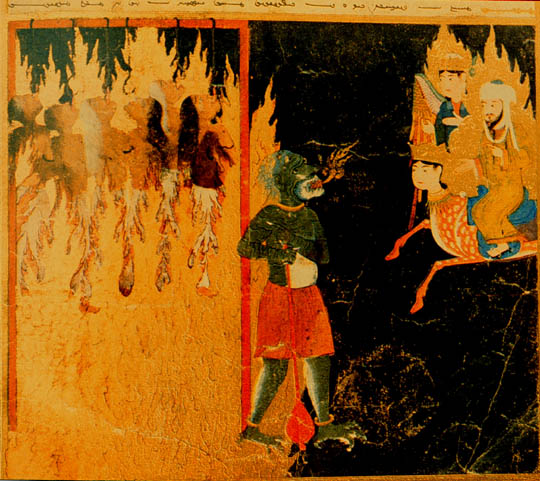
\includegraphics[width=4.07818in,height=3.13349in]{Images/Enfer.jpg}

\vide{les-gardiens-de-lenfer}{%
\paragraph{Les gardiens de
l'enfer}\label{les-gardiens-de-lenfer}}

Chaque strate infernale est gardée par des anges robustes et rudes~:
«~Nous n'avons pris que des anges comme gardiens du Feu~» (S. 74, 31).
«~Des anges gigantesques et puissants se tiendront autour du Feu~; ils
ne désobéissent pas à l'ordre de dieu, ils font ce qui leur est
commandé~» (S. 66, 6). Leurs épaules sont larges. Il faut une année de
marche pour les parcourir. Ils accueillent les damnés par des flammes
aussi volumineuses que les astres. Cette tradition prend sa source
notamment dans la littérature talmudique et dans le Midrash où il est
question des anges gardant les Portes de la Géhenne.

À leur approche l'enfer gronde et mugit. Les damnés épouvantés reculent
à la vue de ces flammes, mais ils sont enchaînés par les anges. Un nuage
fait pleuvoir sur eux non l'eau qu'ils espéraient mais des chaînes. Ils
sont poussés au fond de l'enfer, mais les flammes les remontent~: S. 25,
11-13~: «~Ils ont plutôt qualifié l'Heure de mensonge. Nous avons
cependant préparé, pour quiconque qualifie l'Heure de mensonge, une
Flamme brûlante. Lorsque de loin elle les voit, ils entendront sa fureur
et ses pétillements. Et quand on les y aura jetés, dans un étroit
réduit, les mains liées derrière le cou, ils souhaiteront alors leur
destruction complète~».


\paragraph{Description de l'enfer}\label{description-de-lenfer}

Il y a un feu intense, mais il ne dégage aucune lumière. Un feu noir. Sa
puissance de feu est 70 fois supérieure à celui de la terre. Son
combustible est constitué des damnés dont la chair éternelle alimente
sans cesse le feu de la fournaise. Toutefois, le vendredi, le feu cesse
de brûler. Comme pour l'océan, l'enfer a un rivage. Les réprouvés y
espèrent trouver refuge et tranquillité. Mais ils s'y méprennent car ce
rivage est habité de scorpions énormes, de serpents grands comme des
chameaux. Ils les mordent et s'attaquent aux parties de leurs corps les
plus sensibles~: paupières, lèvres, organes génitaux. Leur venin est si
fort qu'il agit dans le corps 40 années durant. Finalement, ils
préfèrent encore le feu. Le chameau, la brebis ou la vache dont le
propriétaire ne s'est pas acquitté de la \emph{zakāt} sont transformés
en monstres aux cornes et aux sabots de feu qui torturent leurs
propriétaires avares et injustes. Sous les coups, leurs os sont brisés
et leurs crânes fracassés.

 
\paragraph{Les tourments de
l'enfer}\label{les-tourments-de-lenfer}

La figure des damnés sera noire, décharnée, les yeux cautérisés avec des
clous de feu, la langue allongée jusqu'au sol, le front marqué avec du
métal en fusion. Leurs lèvres seront cisaillées en deux par des ciseaux
de feu~; elles repousseront mais seront de nouveau coupées,
éternellement. Leurs bouches vomiront du pus et du sang, de la sanie qui
sera leur propre boisson. Leurs cheveux seront suspendus à des arbres de
feu, leurs entrailles brûleront, leurs dos flagellés par des chaînes de
feu. Pieds et mains enchaînés, ils devront gravir une montagne de feu.

Dans ce monde, leur corps seront plus développés pour qu'ils ressentent
plus encore la douleur. Eux aussi, ils deviennent des monstres. La chair
et la peu feront entendre une voix plus affreuse que le hurlement des
loups.

On trouve en enfer des arbres, les \emph{zaqqūm}. Les réprouvés se
nourrissent de leurs fruits, mais de feu, ils leur brûlent les
entrailles comme du métal en fusion. Plus ils en mangent, plus grande
est leur faim. Ils sont une torture. Ils boivent de l'eau bouillante et
les gardiens leur présentent une coupe débordante de pus et de sanie
bouillonnants qui proviennent de leurs corps. Leurs visages sont
décharnés, brûlés, déchirés. Tout est donc feu, souffrance, torture,
supplice. L'odeur pestilentielle des damnés les conduit à se maudire
mutuellement. C'est alors qu'ils supplient le chef des geôliers, Mālik,
d'intercéder auprès de Dieu pour atténuer leur supplice. Mais ils y
resteront à jamais, à l'exception des croyants grâce à l'intercession
des prophètes.

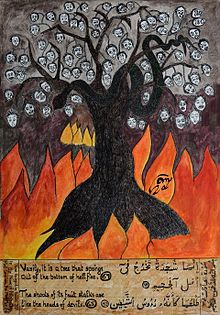
\includegraphics[width=2.73901in,height=2.05312in]{Images/Zaqqum.jpg}


\paragraph{La question de l'éternité des
peines}\label{la-question-de-luxe9ternituxe9-des-peines}

Selon les exégètes traditionalistes, les souffrances sont éternelles.
Une fois plongé dans une de ces demeures, le réprouvé y reste
éternellement. Les ǧahmites qui prétendent que le paradis et l'enfer
sont des accidents et seront donc un jour anéantis sont considérés comme
des innovateurs. Toutefois, on trouve quelques traditionnistes qui
considèrent que seul le Paradis restera éternellement tandis qu'un jour,
l'enfer sera complètement anéanti.

\emph{\textbf{La position des traditionalistes}}

Ils affirment l'éternité de l'enfer et du paradis.

- Cette croyance qui s'appuie sur le consensus, \emph{iǧmā'}, des
compagnons du Prophète et de la première génération. Le consensus est
une des sources du droit musulman avec le Coran et la Sunna.

- Le Coran déclare que les tourments sont perpétuels~«~\emph{ḫalidīn
fîhā 'abadan}~», que les infidèles n'entreront pas au paradis tant que
le chameau n'entre pas dans le trou d'une aiguille~: «~Pour ceux qui
traitent de mensonges Nos enseignements et qui s'en écartent par
orgueil, les portes du ciel ne leur seront pas ouvertes, et ils
n'entreront au Paradis que quand le chameau pénètre dans le chas de
l'aiguille. Ainsi rétribuons-Nous les criminels~» (S. 7, 40). Autrement
dit, aller en enfer, c'est prendre à perpétuité.

- La tradition indique une exception à l'égard des monothéistes
(\emph{muwaḥḥid}) sujets au péché. Grâce à l'intercession des prophètes
ils peuvent sortir de l'enfer. Par suite, les infidèles sont donc quant
à eux condamnés pour toujours.

- Les anciens \emph{al-salaf}, les partisans de la tradition \emph{ahl
al-Sunna}, déclarent la création de l'enfer et du paradis avec ce
monde-ci et ils ne seront jamais anéantis. L'idée d'un anéantissement
est pour eux une innovation.

- C'est une question de justice~: le Coran distingue les fidèles des
infidèles, on ne peut mettre sur le même pied d'égalité les pieux et les
impies. La raison indique que les âmes humaines ont des qualités
immuables. Elles ne peuvent changer leurs conduites antérieures. Elles
ne peuvent donc que subir les peines éternelles.

\emph{\textbf{La critique d'Ibn Al-Qayyim al-Ǧawziyya}}

Célèbre juriste sunnite du quatorzième siècle, commentateur du Coran,
disciple d'Ibn Taymiyya, il procède à une critique de cette
interprétation.

- L'éternité de l'enfer est déjà une question disputée parmi les
compagnons. Il n'y a donc pas consensus. Pour dix des compagnons, nous
ne disposons pas de preuve quant au fait qu'ils aient nié
l'anéantissement de l'enfer. Quant à la première génération, nous
disposons clairement d'opinions controversées.

- Le Coran affirme l'éternité des tourments tant que durera l'enfer.
Tant que l'enfer existe, les infidèles y demeurent. Mais si l'enfer est
anéanti, ses membres en seront délivrés.

- Tant que l'enfer existe, en sortir est le privilège des croyants. Mais
si Dieu détruit l'enfer, les infidèles en seront donc libérés.

- Les traditions n'affirment pas l'éternité de l'enfer en soi~; elles ne
nient pas l'impossibilité de son anéantissement.

- Des compagnons ont déclaré que l'enfer sera anéanti.

- Trois passages coraniques montrent que l'enfer n'est pas éternel~: S.
6, 128~: «~Dieu leur dira: ‹l'Enfer est votre demeure, pour y rester
éternellement, sauf si Allah en décide autrement.› Vraiment ton Seigneur
est Sage et Omniscient~». S. 11, 107~: «~Pour y demeurer éternellement
tant que dureront les cieux et la terre - à moins que ton Seigneur
décide autrement - car ton Seigneur fait absolument tout ce qu'Il veut~»
ou encore~: S. 78, 23~: «~Ils y demeureront pendant des siècles
successifs~». L'éternité de l'enfer dépend donc de la volonté divine, du
Juge Suprême.

- Le Paradis exprime la Miséricorde divine, l'enfer la colère. Or, la
tradition se fait l'écho du triomphe de sa Miséricorde sur sa colère.
Les deux attributs ne sont pas égaux.

- la miséricorde est une fin tandis que la colère est un moyen. L'enfer
n'est qu'un moyen de purification. Un \emph{ḥadīṯ} rapporté par Buḫarî
indique~: «~Dieu a créé la miséricorde et en a multiplié l'aspect. Si
l'Infidèle savait tout ce que Dieu a de miséricorde, il ne désespérerait
jamais d'entrer au Paradis~»\sn{}.

- l'enfer est créé pour menacer les croyants, purifier les pécheurs. La
nature humaine est originellement pure, donc même les infidèles peuvent
être purifiés par le feu. Dieu est tel un médecin qui brûle ou coupe un
membre malade pour guérir l'homme. Il ne se plaît pas au châtiment en
soi. Ce châtiment est un aspect de sa Sagesse, de sa bonté, de sa
justice.

- certaines traditions rapportées par Ibn Hanbal indiquent que celui qui
reconnaît la bonté de Dieu, sa grâce, son pardon, alors l'Enfer devient
pour lui un séjour paisible de rafraîchissement.

- Selon un \emph{hadiṯ qudsi}, la miséricorde de dieu embrasse toutes
choses~: 
\begin{quote}
    «~Je ne fais pas perdre à ceux qui me désobéissent l'espoir de
ma Miséricorde. S'ils reviennent de leur erreur, je suis leur
bien-aimé~; et s'ils ne reviennent pas je suis leur médecin. Je leur
fais subir les peines pour les purifier de leurs erreurs~!~»
\end{quote}


\vide{le-paradis-selon-lislam}{%
\subsection{Le paradis selon l'islam}\label{le-paradis-selon-lislam}}

\vide{existence-localisation-et-duxe9signation}{%
\paragraph{Existence, localisation et
désignation}\label{existence-localisation-et-duxe9signation}}

L'existence du Paradis est affirmée dans le Coran. Selon l'exégèse
traditionnelle, il existe dès à présent, dans un septième ciel. Il a été
créé par Dieu en même temps que notre monde ici-bas comme lieu de
récompense pour les bienheureux (S. 3, 133).

Il existe dans le Coran plusieurs termes pour désigner le paradis.

Le vocable le plus courant est celui de \emph{Ǧanna}, le Jardin. Le
Coran en précise sa nature en évoquant «~le Jardin de la retraite~»
(\emph{Ǧannat al-Ma'wā}, S. 53, 15), le «~Jardin des délices~»
(\emph{Ǧannat an-Na`īm}, S. 10, 9). Il est aussi question du Jardin
d'Eden (\emph{Ǧannat} \emph{`Adn}, S. 61, 12), jardin de bonheur.

Quatre autres expressions sont utilisées pour désigner le paradis~:
\emph{Dâr al-Salām}, la demeure~du salut (S. 6, 127) ; \emph{Dār
al-Muqāma}, la demeure illimitée (S. 35, 35)~; \emph{Dār al-ḫuld}, la
demeure de l'éternité (S. 25, 15) ou encore \emph{dār}
\emph{al-ḥayawān}, la demeure de la vie éternelle (S. 29, 64). On trouve
une autre expression, Firdaws (S. 23, 11) qui est un dérivé du
\emph{Pardes} persan.

\vide{description-du-paradis}{%
\paragraph{Description du
paradis}\label{description-du-paradis}}

Les descriptions du Paradis sont nombreuses et la littérature
\emph{ḥadīṯ} en donne des images empruntes d'une grande sensualité et
beauté. Il est question d'un lieu de palais aux voutes de perles, de
tapis de fleurs, d'arbres aux couleurs jusqu'alors inconnues des hommes,
les jujubiers d'al-\emph{Muntahā}.
\begin{quote}
    S. 4, 57~: «~Et quant à ceux qui ont cru et fait de bonnes œuvres,
bientôt Nous les ferons entrer aux Jardins sous lesquels coulent des
ruisseaux. Ils y demeureront éternellement. Il y aura là pour eux des
épouses purifiées. Et Nous les ferons entrer sous un ombrage épais».
\end{quote}


On y trouve des fleuves comme dans le paradis terrestre de la Genèse,
mais il n'y coule pas seulement de l'eau~:
\begin{quote}
    «~Il y aura là des fleuves dont l'eau est incorruptible, des fleuves de
lait au goût inaltérable, des fleuves de vin, délices pour ceux qui en
boivent, des fleuves de miel purifié. Ils y trouveront aussi toutes
sortes de fruits et le pardon de leur Seigneur (S. 47, 15)~».
\end{quote}


Cette description rappelle la description de la Terre promise aux
Hébreux dans l'Ancien Testament. Elle était désignée comme une terre où
ruissellent le lait et le miel (Ex 3, 8, 17 ou Ex 13, 5~; Deut 6, 3,
etc.). C'est un pays d'abondance, de source d'eau, de vigne\ldots Le
2\textsuperscript{ème} Livre d'Hénoch et l'Apocalypse de Paul évoquent
aussi les ruisseaux de miel, de lait, de vin et d'huile.

Il y a des vierges éternelles~:
\begin{quote}
    «~ Là, il y aura des vertueuses et des belles.\\
Lequel donc des bienfaits de votre Seigneur nierez-vous~?\\
Des houris cloîtrées dans les tentes,\\
Lequel donc des bienfaits de votre Seigneur nierez-vous~?\\
qu'avant eux aucun homme ou djins n'a déflorées.\\
Lequel donc des bienfaits de votre Seigneur nierez-vous~?\\
Ils seront accoudés sur des coussins verts et des tapis épais et
jolis.\\
Lequel donc des bienfaits de votre Seigneur nierez-vous~? (S. 55,
70-77)~».
\end{quote}


Et des éphèbes : 
\begin{quote}
    «~ Parmi eux circuleront des garçons éternellement
jeunes,\\
avec des coupes, des aiguières et un verre (rempli) d'une liqueur de
source\\
qui ne leur provoquera ni maux de tête ni étourdissement;\\
et des fruits de leur choix,\\
et toute chair d'oiseau qu'ils désireront.\\
Et ils auront des houris aux yeux, grands et beaux,\\
pareilles à des perles en coquille\\
en récompense pour ce qu'ils faisaient (S. 56, 17-24) ».
\end{quote}

On peut y boire du vin car il n'enivre pas~:
\begin{quote}
   «~On leur sert à boire un nectar pur, cacheté, laissant un arrière-goût
de musc.

Que ceux qui la convoitent entrent en compétition (pour l'acquérir)\\
Il est mélangé à la boisson de Tasnīm,\\
source dont les rapprochés boivent (S. 83, 25-28)~». 
\end{quote}


Ce qui est à relever dans ces descriptions, c'est l'atmosphère de
banquet qui y règne. Les élus sont accoudés sur des tapis aux revers de
brocart\ldots{} sur des coussins verts et sur de beaux tapis (S. 55, 54
et 76), ils boivent un vin délectable. Ces images sont typiques de la
tradition juive qui sert à décrire le bonheur des justes.

\vide{accuxe8s-au-paradis}{%
\paragraph{Accès au paradis}\label{accuxe8s-au-paradis}}

Le Paradis est constitué de différents étages. La tradition distingue
huit portes qui ouvrent à différents espaces paradisiaques et qui
s'ouvrent en fonction des actions accomplies par les croyants. Il y a
ainsi la porte de la prière, de la guerre sainte, de l'aumône, du jeûne,
du repentir, des patients (ceux qui maîtrisent leur colère), de la
soumission à la volonté divine, enfin la porte droite celle qui ne
nécessite pas de jugement préalable~: c'est elle qu'emprunte Muḥammad.

Il est nécessaire pour entrer au paradis d'avoir un laisser passer et
selon une tradition, chaque croyant entrera au paradis avec un passeport
sur lequel sera indiqué~: 
\begin{quote}
    «~Au nom de Dieu, le Bienfaiteur, le
Miséricordieux. Nous délivrons à \ldots{} fils de\ldots{} un permis
d'entrée au jardin sublime, dont les fruits à cueillir seront à portée
de sa main~».
\end{quote}

Les élus sont accueillis par un chœur d'anges qui chante en arabe, ils
ont un visage radieux après avoir été lavés dans une douce fontaine.

Le climat du Paradis est doux~: «~Il n'y sévit ni la chaleur du soleil,
ni la rigueur du froid (S. 75, 3). Les mois comprennent 500
jours\ldots{} et les années 500 mois.

\vide{les-uxe9lus}{%
\paragraph{Les élus
}\label{les-uxe9lus}}

Ils ont l'apparence d'un homme âgé de 33 ans, ils sont imberbes.

Toute épouse vierge au moment du mariage sera la femme légitime du
Bienheureux au paradis. Le Bienheureux qui a eu plusieurs épouses les
gardera toutes. Si la femme a eu plusieurs maris, elle se consacrera au
dernier, au meilleur ou à celui de son choix.

\vide{la-question-des-femmes-au-paradis}{%
\paragraph{La question des femmes au
paradis}\label{la-question-des-femmes-au-paradis}}

Mais justement, revenons sur la question de la femme.

Le Coran est explicite quant à l'égale possibilité pour les hommes et
les femmes d'accéder au paradis ou en enfer~:
\begin{quote}
    «~Et quiconque, homme ou femme, fait de bonnes oeuvres, tout en étant
croyant... les voilà ceux qui entreront au Paradis; et on ne leur fera
aucune injustice, fût-ce d'un creux de noyau de datte~» (S. 4, 124).



«~{[}Il en est ainsi{]} afin qu'Allah châtie les hypocrites, hommes et
femmes, et les associateurs et les associatrices, et Allah accueille le
repentir des croyants et des croyantes. Allah est Pardonneur et
Miséricordieux~» (S. 33, 73).
\end{quote}
Il semble cependant qu'il y ait en enfer plus de femmes que d'hommes.
Ceci est indiqué dans un \emph{ḥadīṯ} alors que Muḥammad eut une
vision~: 
\begin{quote}
    «~J'ai vu le feu et je n'ai pas vu à ce jour un spectacle plus
terrible. La plupart des habitants sont des femmes~». la raison en est
leur ingratitude, leur manque de charité, leur négativité dans le regard
des actions conduites par leurs maris~: «~si les hommes font de bonnes
choses, la femme voit une chose mauvais, et vous dit qu'elle n'a jamais
rien vu de bon du tout~» (Ahmad ibn Hanbal, I.359, cité dans Smith et
Haddad 1975: 44).
\end{quote}


Le Coran mentionne les femmes de Lot et de Noé qui à cause de leur
trahison furent conduites au Feu. Leurs saints maris ne leur furent
d'aucun secours~: 
\begin{quote}
    «~Allah a cité en parabole pour ceux qui ont mécru la
femme de Noé et la femme de Lot. Elles étaient sous l'autorité de deux
vertueux de Nos serviteurs. Toutes deux les trahirent et ils ne furent
d'aucune aide pour {[}ces deux femmes{]} vis-à-vis d'Allah. Et il
{[}leur{]} fut dit: ‹Entrez au Feu toutes les deux, avec ceux qui y
entrent~» (S. 66, 10).
\end{quote}


Notons que parmi les signes de la venue du jugement dernier, on trouve
mentionné le renversement des valeurs morales traditionnelles entre
l'homme et la femme~: l'homme doit obéir à sa femme et il désobéit à ses
parents, l'homme doit travailler pour sa femme, les femmes vont au
pèlerinage ensemble sans être accompagnées d'un homme, il y a une pleine
licence sexuelle. Le nombre d'homme décroît tandis qu'il y a cinquante
femmes pour un homme.

\vide{la-question-des-houris}{%
\paragraph{La question des
houris}\label{la-question-des-houris}}

Houris vient du mot arabe \emph{ḥawrâ'}, pluriel de \emph{ḥur.}

\emph{Le Coran} mentionne à plusieurs reprises les houris~:
\begin{quote}
   S. 44, 54~: «~C'est ainsi! Et Nous leur donnerons pour épouses des
houris aux grands yeux~». 
S. 55, 56~: «~Ils y trouveront {[}les houris{]} aux regards chastes,
qu'avant eux aucun homme ou djinn n'aura déflorées~».

S. 52, 20~: «~accoudés sur des lits bien rangés›, et Nous leur ferons
épouser des houris aux grands yeux noirs~».

S. 55, 72~: «~des houris cloîtrées dans les tentes~».

S. 56, 22~: «~Et ils auront des houris aux yeux, grands et beaux~»
\end{quote}




Quant au ḥadīṯ, on trouve dans la compilation de al-Buḫarî~\sn{Livre 54, \emph{Le commencement de la création}, ḥadīṯ 476.}:
\begin{quote}
    Le Prophète a dit: «Les premières personnes qui entreront au paradis
seront brillantes comme la pleine lune, et les suivantes brillantes
comme l'étoile la plus brillante dans le ciel. Leurs cœurs seront comme
le cœur d'un seul homme, car ils n'auront ni haine ni jalousie entre
eux, tout le monde aura deux épouses, des houris, qui seront aussi
belles, pures et transparentes que la moelle des os de leurs jambes~»

\end{quote}


Autre hadîth de Buḫari~: rapporté par Abu Huraira: 
\begin{quote}
    «~L'Apôtre d'Allah
dit: «Les premières personnes à entre au paradis, seront brillantes
comme la pleine lune et celles qui les suivront, brilleront comme
l'étoile la plus brillante dans le ciel. Ils n'urineront pas, ils ne se
soulageront pas, ils ne cracheront pas et n'auront pas de sécrétions
nasales. Leurs peignes seront d'or, et leur sueur d'une odeur de musc.
Leurs épouses seront des houris. Elles ressembleront toutes à leur père
Adam (dans leur état), elles seront grandes de soixante coudées de
hauteur~».
\end{quote}


\paragraph{Les commentateurs}

Elles ont suscité plusieurs questions

\begin{itemize}
\item
  sont-elles de la même essence que les femmes~?
\item
  sont-elles de la lignée d'Eve~?
\item
\end{itemize}

Pour certains commentateurs, elles ont été créées de safran. Mais elles
semblent bien être faites de chair. Leur luminosité y est dépeinte dans
un style hyperbolique~: leurs sourcils ressemblent à un trait noir placé
sur de la lumière et leur front rappel un croissant de lune.

Les commentateurs se sont aussi interrogés sur les délices qu'elles
peuvent procurer aux croyants~? Combien de houris un Croyant peut-il
honorer de ses faveurs par nuit~? Des réponses diverses qui montrent
cependant que l'occupation principale au paradis sera de s'enlacer de ces
femmes vierges. Et le plaisir de l'homme y sera décuplé de 100 fois de
celui sur terre. Elles attendent au ciel leurs époux et maudissent leurs
femmes terrestres lorsque celles-ci se fâchent ou les contrarient leurs
maris.

Les houris sont pures. Elles ne souffrent des aléas de la menstruation,
elles n'éprouvent aucune fatigue. Les élus mangent les fruits délicieux
du paradis par pure jouissance. Les résidus de la digestion se
transforment en une exhalation parfumée du corps.

\paragraph{L'hypothèse syriaque}

En l'an 2000, un chercheur libanais-allemand sous le pseudonyme de
Christoph Luxenberg a publié un ouvrage intitulé \emph{Die
Syro-Aramäische Lesart des Koran:~ Ein Beitrag zur Entschlüsselung der
Koransprache} \sn{en français~: \emph{Lecture syro-araméenne du Coran~: une
contribution pour décoder la langue du Coran}}. Cet ouvrage est une
étude philologique qui met en lumière l'existence particulière d'une
source du Coran. Si nombreux sont les auteurs qui ont souligné
l'influence des textes bibliques, Luxenberg indique l'adoption plus
particulière d'un lectionnaire syriaque, et plus particulièrement d'un
ouvrage liturgique à vocation ce missionnaire. Ces travaux poursuivent
l'enquête menée par Günther Lulling.

Sa méthodologie consiste à rechercher les équivalents syriaques des
termes arabes et de clarifier le sens de certains passages coraniques
obscurs à l'aide des termes syriaques.

À cet égard, le mot houri signifierait non pas une vierge aux grands
yeux noirs, mais du raisin blanc.

\vide{conclusion-la-vision-de-dieu}{%
\section{{Conclusion~: La vision de Dieu
}}\label{conclusion-la-vision-de-dieu}}

La question de la vision de Dieu n'est pas étrangère à la tradition
musulmane. Elle y est affirmée parfois de manière explicite~: Chaque
vendredi, hommes et femmes rendent visite au Seigneur sur son
invitation. Chemin faisant, ils passent devant le tableau du Destin,
\emph{al-Lawḥ al-mahfūẓ} où se trouvent consignées toutes les actions
des êtres. Sur des montures ailées, les Bienheureux parviennent en un
clin d'œil devant le Trône du Tout-Puissant. Le voile de lumière se lève
et l'Eternel paraît. La voix divine retentit~: «~al-salām alaykum~». La
vue de Dieu surpasse tous les délices du paradis.

Si l'ensemble de ces descriptions sont marquées par une très grande
sensibilité, il ne faut pas oublier, à l'exemple du cours sur la
philosophie, qu'elles ont donné lieu à des interprétations et à une
lecture spirituelle. Ainsi, al-Ġazālī soutient que la vision de Dieu
relève de l'ordre de la connaissance~: voir Dieu, c'est accéder non à
une vision physique, mais à sa connaissance.
